\chapter{Cellular Technology}
\label{chpt:celltech}
\section{Introduction}
In the information age we currently live in almost every device has a wireless technology of sort that it uses to provide a specific service. Radios for audio entertainment; television remotes to change 
channels; cellular phones for communication; wireless access points to create wireless LAN's\cite{Karen2004}. Wireless technology is now part of our everyday life.

The popularity and rapid adoption of wireless technology has made it difficult to plan,manage and operate wireless networks. Wireless technology facilitates communication between two entities by transmitting data or voice via a radio frequency. 

As the popularity and use of services that use wireless technology increase, the greater the need for these services to use different radio frequencies to communicate. This need arises due to an effect called \emph{interference} which occurs when two or more connections between entities use the same radio frequency to facilitate communication. This effect is discussed in more detail in Chapter 3.

Therefore the use of frequencies by services must be carefully considered to avoid interference when entities communicate with each other, which is a problem since the amount of entities that communicate far out strip the amount of frequencies available for communication. Thus assigning frequencies to entities for communication is a difficult problem and refered to as the frequency assignment problem (FAP).

Initially manual techniques were used to assign frequencies in an attempt to solve the FAP. But as a result, the assignment of frequencies was either to complex or just too daunting because of shear amount of entities that need to be assigned frequencies. Also, because of the rapid adoption of wireless technology the assignment of frequencies needed to be dynamic and hence, automated.

When a task needs to be automated an algorithm needs to be developed to tell the machine how it must go about to solve the problem it is destined to work on. Early algorithms developed to solve the FAP utilized brute force\footnote{Brute force refers to a method which sequentialy tries every possible combination in hope of finding a solution} techniques to assign frequencies.

Since the FAP is proven to be NP-Hard problem, thus using an algorithm that tries to brute force a solution is futile as no solution can be found in a reasonable time frame. Hence, algorithms based on heuristic techniques are utilized in an attempt to either solve the FAP or come close to a solution. Heuristic Algorithms will be discussed in Chapter 4.

In this chapter we start by discussing GSM as well as a brief history of GSM. The topology of GSM is then explained before moving onto the problems in that are present GSM network. One of the major problems being the FAP.

\section{GSM Networks}
The General System for Mobile Communications (GSM) is a system for multi-service cellular communication which is capable of providing voice as well as data services. Most cellular networks in operation 
are GSM based. The primary service that GSM caters for is voice communication, but other data services such as Short Message Service (SMS), Multimedia Message Service (MMS) and Internet 
connectivity services such as \emph{general packet radio system} (GPRS),\emph{enhanced data rate for global evolution} (EDGE) and \emph{high speed circuit switched data} (HSCSD) are becoming more important\cite{GSMArchitectureProtocolsServices,Eisenblatter}.

GSM is one of the most widely used radio communications technologies, which is why we need to look at the history behind it in order for us to understand the domain of radio communication better \cite{GSMArchitectureProtocolsServices}. A brief history of the GSM network specification will now be presented in the next section.

\subsection{A Brief History of GSM Networks}
In the early 1981 a group known as the Groupe Speciale Mobile (GSM) was established to develop a Europe wide radio communication system using the reserved 900 MHz band\footnote{In 1990 the United Kingdom requested that 1800MHz band be added to the scope of the GSM standard group. This variant of the GSM specification became known as the \emph{Digital Cellular System 1800} (DCS1800) \cite{GSM92}.}.

At the start of the GSM specification in the early 1980's it was initially thought that the system would be analogue based, but this soon changed with the \emph{integrated service digital network} (ISDN) specification nearing completion. As such the GSM specification started following much of the same design principles and access protocols that ISDN exhibited.

After the completion of the ISDN specification and the advantages of switching to digital instead of analogue for communication became clear. One of the primary advantages of ISDN is that it is capable of transmitting data as higher speeds. GSM would therefore be based on digital transmission and speech would be represented by a digital stream of 16 kbits/s \cite{GSM92}.

The primary benefit that one can deduce from the use of ISDN over slower analogue connections is because data can be transmitted faster, more data can be sent for the same amount of time it would've taken on an analogue connection. Hence, since more data can be sent it has the net effect of increasing the quality and efficientcy of the connection between two entities, the network therefore does not need to remove as much information from a packet to be sent to fit within the data transmission constraints.

Before the switch to digital transmission was finalized the GSM first wanted to evaluate the spectral efficiency of analogue and digital based transmission. Spectral efficiency plays an important part in wireless communication since the radio spectrum is a limited resource and whichever transmission technology is used, the utilization of the spectrum should be maximised. 

Maximum utilisation is an important problem which we will discuss in detail in later sections of this chapter. After an evaluation on sepctrail efficiency it was finalized that the GSM system would be digital based using \emph{time division multiple access} (TDMA) \cite{GSM92,GSMSysEngin}.

By the early 1990’s GSM became an evolving standard and the first GSM based network was demonstrated in 1991\footnote{Near the end of 1991 the GSM group was renamed to \emph{Speciale Mobile Group} (SMG) to eliminate confusion with the standard and the group.}. The following year a number of GSM networks were operating in Europe due to mobile terminals / equipment capable of operating on the networks becoming more widely available to the general public. In the same year an operator in Australia became the first non-European operator to implement a GSM based network\cite{Eisenblatter}.

The collective subscriber base of GSM networks surpassed the million subscriber mark in 1993. Due to this phenomenal growth in GSM network use, numerous extensions were made to the GSM specification. 
Some of the extensions that were made are the following\cite{Eisenblatter}:
\begin{itemize}
\item Half rate speech telephony
\item Improved SMS
\item Line Identification
\item Call waiting
\item Call holding
\end{itemize}
The specification with these extensions defined is known as the GSM Phase 2. As the world shifted towards more digital and data intensive services it became difficult to deliver these services over GSM networks. This difficulty was due to the restriction that data could only be transmitted at 9.6 Kbps \cite{GSM92}.

The new specification defined new technologies such as GPRS,EDGE and HSCSD which were designed with the primary goal of making more bandwidth available for data transmission \cite{GSMArchitectureProtocolsServices}. Data transmission was improved by these technologies by enabling that more than one GSM slot be used for a terminal or service at a time\cite{GSMArchitectureProtocolsServices}.

By enabling that more than one GSM slot be used by a terminal or service, tranceivers are required to have a higher signal to noise ratio \cite{GSMArchitectureProtocolsServices}. This requirement has an impact that effects radio interfaces as there is a higher likelyhood that interference might occur, hence it makes it more difficult to generate a low interference Freuqnecy plan \cite{Eisenblatter}. 

The actual signal to noise ratio at a receiver is dependent on a number of factors that include \cite{GSMArchitectureProtocolsServices,Karen2004}:
\begin{itemize}
\item Frequency used at the transceiver
\item Strength of the signal
\item Weather conditions
\item Shape of the surrounding environment
\item Direction of the transmission
\end{itemize}
Even taking these factors into account the calculation of the signal to noise ratio at a transceiver is not trivial. For a more in depth discussion on the calculation the reader is directed at the survey by \cite{Karen2004}.

As the GSM standard matured as a cellular technology, industry experts already began specification of the next generation of cellular networks which would in time, replace the GSM cellular system. 

The \emph{Universal Mobile Telecommunications System} (UMTS) can be considered the 3rd generation (3G) of cellular networks. UMTS was designed from the beginning to operate in parallel with the legacy GSM system. The first standard of the UMTS was issued in the beginning of 2000 and subsequently most modern networks are based on it or are migrating their networks to it.

UMTS is a large improvement of the GSM in two areas namely Data Transmission bandwidth and Frequency Planning due to UMTS utilising \emph{DS-CDMA} (direct sequence code division multiple access) and \emph{WCDMA} (Wide Band Code Division Multiple Access). The higher data transmission speed (2 Mb/s) can be attributed to UMTS using the DS-CDMA scheme. The scheme also allows more users to be served than previous generation of networks\cite{tabuglobalplanning3g,Eisenblatter}. 

A direct consequence of UMTS utilizing DS-CDMA and WCDMA, which sends data over a wide-band of 5 Mhz, therefore no frequency planning problem comparable to GSM has to be solved\cite{tabuglobalplanning3g,Eisenblatter}. 

\emph{Code division multiple access} (CDMA) is a technology primarily used in broadband systems. Users do not gain access to only a small portion of the bandwith, but rather use the entire band for the duration of a connection. Users also do not gain exclusive access to the whole band, but instead share the usage of the bandwith with other users simultaneously, hence the name \emph{multiple access}. Users using a band simultaneously are seperated using orthogonal codes \cite{GSMArchitectureProtocolsServices}.

With CDMA a users signal is not transmitted as its original signal. Instead the signal is spectrally spread over a mutiple of its original bandwith using a spreading factor \cite{GSMArchitectureProtocolsServices}. The spreading factor fluctuates between values of 10 and 1000 \cite{GSMArchitectureProtocolsServices}. Using these spreading factors less interference and distrubances are encountered because the broadband signal is generated from a narrowband signal \cite{GSMArchitectureProtocolsServices}.
UMTS may be a large improvement, but its adoption does not spread very far from busy city centres which contain a large concentration of clients in a small geographical area. The reason for this is that, as mentioned previously, UMTS caters for larger data usage and therefore more clients can be serviced simultaneously \cite{GSMArchitectureProtocolsServices}.

Most network operators do not implement entirely new backbone architecture for UMTS to operate on but instead, utilize the same backbone used for GSM and GPRS. This not only extends the lifetime of previous infrastructure investment by the operator but also builds upon the redundancy provided by the GSM network \cite{GSMArchitectureProtocolsServices}. Thus even with new technological improvements such as UMTS, GSM as a wireless technology is still used for communication and is therefore still relevant today.

In this section a brief overview of the history of the GSM Network specification was given. In the next section an explanation of the topology of GSM network will be given. This will broad the understanding behind GSM networks.

\begin{figure}[hptb]
	\begin{centering}
		\documentclass[11pt]{article}
\usepackage{tikz}
\usepackage{xcolor}

\begin{document}
	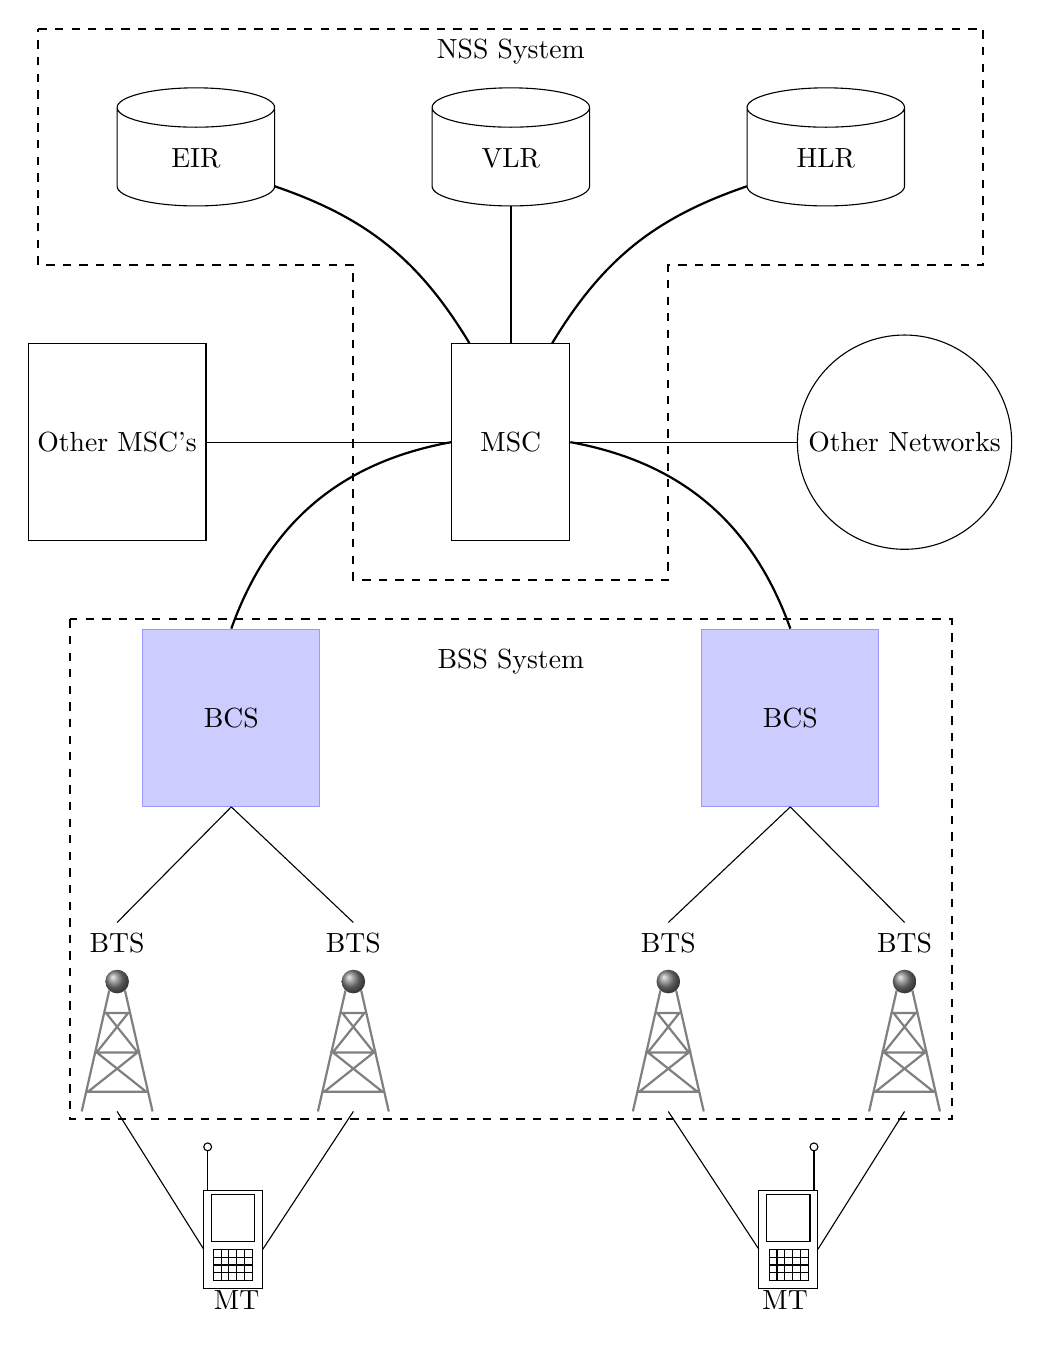
\begin{tikzpicture}[scale=1.0]
		%\draw[step=0.25cm,thin,color=gray] (-6,-8) grid (6,8);
		%drawing of handsets
		%left handset
		\draw (-3.85,-6.20) circle (0.05cm);
		\draw (-3.85,-6.75) -- (-3.85,-6.25);
		\draw (-3.9,-8) node [below=0.15cm,right=0.005cm] {MT} rectangle (-3.15,-6.75);
		\draw (-3.8,-7.4) rectangle (-3.25,-6.8);
		\foreach \x in {0.0,0.1,0.2,0.3,0.4}
		{
			\foreach \y in {0.0,0.1,0.2,0.3}
			{
				\draw (-3.78 + \x,-7.6 - \y) rectangle (-3.68 + \x,-7.5 - \y);
			}
		}
		%right handset
		\draw (3.85,-6.20) circle (0.05cm);
		\draw (3.85,-6.75) -- (3.85,-6.25);
		\draw (3.9,-8) node [below=0.15cm,left=0.005cm] {MT} rectangle (3.15,-6.75);
		\draw (3.8,-7.4) rectangle (3.25,-6.8);
		\foreach \x in {0.0,0.1,0.2,0.3,0.4}
		{
			\foreach \y in {0.0,0.1,0.2,0.3}
			{
				\draw (3.38 + \x,-7.6 - \y) rectangle (3.28 + \x,-7.5 - \y);
			}
		}
		%Drawing of the BTS's
		\begin{scope}
			\foreach \x in {-5,-2,2,5}
			{
				\path (\x,-4.1) coordinate (TowerCirlce);
				\path (\x - 0.10,-4.215) coordinate (startLeftMast);
				\path (\x + 0.10,-4.215) coordinate (startRightMast);
				\path (\x - 0.45,-5.75) coordinate (endLeftMast);
				\path (\x + 0.45,-5.75) coordinate (endRightMast);
				\path (\x - 0.140,-4.5) coordinate (startTopHorizontalBar);
				\path (\x + 0.140,-4.5) coordinate (endTopHorizontalBar);
				\path (\x - 0.260,-5) coordinate (startMiddelHorizontalBar);
				\path (\x + 0.260,-5) coordinate (endMiddelHorizontalBar);
				\path (\x - 0.370,-5.5) coordinate (startBottomHorizontalBar);
				\path (\x + 0.370,-5.5) coordinate (endBottomHorizontalBar);
						\draw [thick,color=gray] (startLeftMast) -- (endLeftMast) (startRightMast) -- (endRightMast) (startMiddelHorizontalBar) -- (endTopHorizontalBar) -- (startTopHorizontalBar) -- (endMiddelHorizontalBar) -- (startMiddelHorizontalBar) -- (endBottomHorizontalBar) -- (startBottomHorizontalBar) -- (endMiddelHorizontalBar) -- cycle;
					\shade [ball color=gray] (TowerCirlce) circle (0.15) node [above=0.25cm] {BTS};
			}
		\end{scope}
		%Lines connecting Handsets with BTS's
		%Left
		\draw (-5,-5.75) -- (-3.9,-7.5);
		\draw (-2,-5.75) -- (-3.15,-7.5);
		%Right
		\draw (5,-5.75) -- (3.9,-7.5);
		\draw (2,-5.75) -- (3.15,-7.5);
		%Drawing of BCS's
		\begin{scope}
			\node (LeftBCS) at (-3.55,-0.75) [shape=rectangle,draw=blue!40, fill=blue!20,minimum size = 2.25cm] {BCS};
			\draw (LeftBCS.south) -- (-5,-3.35);
			\draw (LeftBCS.south) -- (-2,-3.35);
			\node (RightBCS) at (3.55,-0.75) [shape=rectangle,draw=blue!40, fill=blue!20,minimum size = 2.25cm] {BCS};
			\draw (RightBCS.south) -- (5,-3.35);
			\draw (RightBCS.south) -- (2,-3.35);
			\draw [dashed,thick,color=black] (-5.6,0.5) rectangle (5.6,-5.85) (0,0.25) node [anchor=north] {BSS System};
		\end{scope}
		%Draw MSC
		\node (MiddelMSC) at (0,2.75) [shape=rectangle,draw=black,minimum height=2.5cm, minimum width=1.5cm] {MSC};
		\draw [thick] (MiddelMSC.west) to [bend right=30] (LeftBCS.north);
		\draw [thick] (MiddelMSC.east) to [bend left=30] (RightBCS.north);
		\node (LeftMSC) at (-5,2.75) [shape=rectangle,draw=black,minimum height=2.5cm, minimum width=1.5cm] {Other MSC's};
		\node (OtherNetworks) at (5,2.75) [shape=circle,draw=black] {Other Networks};
		\draw (LeftMSC.east) to (MiddelMSC);
		\draw (MiddelMSC) to (OtherNetworks);
		%Databases
		\draw (0,7) circle (1cm and .25cm) node [below=0.40cm] {VLR} ++ (-1,-1) arc (180:360:1cm and .25cm) ++ (-2.0,1) -- (-1.0,6) ++ (2.0,1) -- (1.0,6);
		\draw (-4,7) circle (1cm and .25cm) node [below=0.40cm] {EIR} ++ (-1,-1) arc (180:360:1cm and .25cm) ++ (-2.0,1) -- (-5.0,6) ++ (2.0,1) -- (-3.0,6);
		\draw (4,7) circle (1cm and .25cm) node [below=0.40cm] {HLR} ++ (-1,-1) arc (180:360:1cm and .25cm) ++ (-2.0,1) -- (3.0,6) ++ (2.0,1) -- (5.0,6);
		\draw[thick] (-3,6) to [bend left=20] (MiddelMSC);
		\draw[thick] (0,5.75) to (MiddelMSC);
		\draw[thick] (3,6) to [bend right=20] (MiddelMSC);
		\draw[dashed,thick,color=black] (-6,8) -- (0,8) node [anchor=north] {NSS System} -- (6,8) -- (6,5) -- (2,5) -- (2,1) -- (-2,1) -- (-2,5) -- (-6,5) -- (-6,8) -- cycle;
	\end{tikzpicture}
\end{document}

		\caption{GSM Architecture}
		\label{fig:GSMArchitecture}
	\end{centering}
\end{figure}

\section{Topology of a GSM Network}
GSM networks consists of a variety of different subsystems to realise the goal of establishing a radio communication link between two parties. The hierarchy of systems and their respective connections to each other is illustrated in figure \ref{fig:GSMArchitecture}. Each subsystem will now be discussed.
\subsubsection{Mobile Station (MS)}
A Mobile station (MS) as it is defined in the GSM specification refers to any mobile device that is capable of of making and receiving calls on a GSM network.  The MS is the main gateway 
for a user to gain access to the GSM network \cite{Eisenblatter,GSMArchitectureProtocolsServices}. Typical devices that fall under the category of MS are Cellular Phones, Smart Phones and POS devices. The MS has two features which play an important role throughout the GSM Network, namely:
\begin{description}
\item[Subscriber Identification Module (SIM)] --- Usually inserted into a mobile devices. The SIM contains the \emph{international mobile subscriber identity} (IMSI) and is used throughout the network for authentication as well as being a key part in providing encrypted transmissions \cite{Eisenblatter}.
\item[International Mobile Equipment Identity(IMEI)] --- Used to identify mobile station equipment. Primarily used in the denial of service to equipment that has been blacklisted\footnote{Equipment can be blacklisted for a variety of reasons e.g. theft} and tries to gain access to the network \cite{Eisenblatter}.
\end{description}
The MS has the capability to change the transmission power it uses from its base value to a maximum value of 20 mW. The change in transmission power is automatically set to the lowest level by the base transceiver station (BTS) to ensure reliable communication after evaluating the signal strength as measured by the MS \cite{GSMSysEngin,GSMArchitectureProtocolsServices}. The power adjustment also minimizes cochannel interference because the transmitted signal is less powerful therefore less likely to interfere with other signals\cite{GSMSysEngin}.

\subsection{Base Station Subsystem (BSS)}

According to the GSM Phase 2+ specification this system is viewed by the \emph{mobile switching centre} (MSC) through an Abis radio interface as the system responsible for communicating with mobile stations in a particular location area. The BSS usually consists of one \emph{base station controller} (BSC) with one or more \emph{base transceiver stations} (BTS) which it controls. The communication link between the MSC and BSC is the called the A-interface and the communication link between the BSC and BTS is called the Abis interface. A BTS has similar equipment to that of a Mobile Station. Both have transceivers, antennas and the necessary functions to perform radio communication. 

In a GSM network the Service Area (SA) is subdivided into Location Areas(LA's) which are then futher divided into smaller radio zones called cells \cite{GSMSecurInTeleNetwork}. 

When a cellular network is modeled, cells are modeled as hexagonal shapes. Each cell in the modelled network is served by only one BTS and is usually regarded to be in the center of a cell as can be seen in figure \ref{fig:GSMCell}\cite{GSMArchitectureProtocolsServices}. Even though cells are modelled as being hexagons (see figure \ref{fig:GSMCell}) the actual coverage area of a cell has no predefined regular shape \cite{GSMArchitectureProtocolsServices}.

With the network modelled as a series of interconnecting hexagons it allows one to more easily take constraints into account. For a cell to serve its geographical area, it needs to be allocated frequencies to operate on. Therefore, for each cell $i$ in the modelled network a subset $S_i$ of frequencies from the total frequencies $F$ allocated to the GSM network is assigned\cite{GSMArchitectureProtocolsServices}. Neighboring cells must at all cost avoid having the same subset of frequencies allocated to them, since such a scenario would lead to severe interference on any communication and thus degrade quality \cite{GSMArchitectureProtocolsServices}.

Since the amount of cells in a network greatly outnumber the availbe of subset frequencies available one is forced to start reusing frequency subsets in cells. To ensure the resused frequency subsets do not interfere with their neighboring cells a reuse distance $D$ is defined \cite{GSMArchitectureProtocolsServices}. Which basically means that a certain amount of cells must be between the cell already assigned the frequency subset $S_i$ and the cell to be assigned a frequency subset \cite{GSMArchitectureProtocolsServices}. The amount of cells is the distance value $D$.

A cell is divided into 1 to 3 service sectors and each sector is allocated an antenna/transceiver \cite{GSMSysEngin}. Depending on how many sectors are at a cell, the operating angle of the antennae needs to be adjusted accordingly to ensure 360 degree service. If there is only one sector an omni-directional antenna is used, otherwise the antennae operating angle are adjusted to $\frac{360\,^{\circ}}{n}$ where ${n}$ is the amount of antennae \cite{Eisenblatter}.
\begin{figure}[h]
	\begin{centering}
		\begin{tikzpicture}
	%===============================Top======================================
	\node [regular polygon, regular polygon sides=6, minimum size=3cm,draw] at (0,1) {};
	\path (0,1.75) coordinate (TowerCirlce);
	\path (0 - 0.10,1.635) coordinate (startLeftMast);
	\path (0 + 0.10,1.635) coordinate (startRightMast);
	\path (0 - 0.45,0.01) coordinate (endLeftMast);
	\path (0 + 0.45,0.01) coordinate (endRightMast);
	\path (0 - 0.140,1.345) coordinate (startTopHorizontalBar);
	\path (0 + 0.140,1.345) coordinate (endTopHorizontalBar);
	\path (0 - 0.260,0.85) coordinate (startMiddelHorizontalBar);
	\path (0 + 0.260,0.85) coordinate (endMiddelHorizontalBar);
	\path (0 - 0.370,0.35) coordinate (startBottomHorizontalBar);
	\path (0 + 0.370,0.35) coordinate (endBottomHorizontalBar);
	\draw [thick,color=gray] (startLeftMast) -- (endLeftMast) (startRightMast) -- (endRightMast) (startMiddelHorizontalBar) -- (endTopHorizontalBar) -- (startTopHorizontalBar) -- (endMiddelHorizontalBar) -- (startMiddelHorizontalBar) -- (endBottomHorizontalBar) -- (startBottomHorizontalBar) -- (endMiddelHorizontalBar) -- cycle;
	\shade [ball color=gray] (TowerCirlce) circle (0.15) node [above=0.10cm] {\tiny{BTS}};
	%%========================================================================
	%%================================Second Line======================================
	\foreach \x in {-2.25,2.25}
	{
		\node [regular polygon, regular polygon sides=6, minimum size=3cm,draw] at (\x,-0.3) {};
		\path (\x,-0.3 + 0.75) coordinate (TowerCirlce);
		\path (\x - 0.10,-0.3 + 0.635) coordinate (startLeftMast);
		\path (\x + 0.10,-0.3 + 0.635) coordinate (startRightMast);
		\path (\x - 0.45,-0.3 - 0.99) coordinate (endLeftMast);
		\path (\x + 0.45,-0.3 - 0.99) coordinate (endRightMast);
		\path (\x - 0.140,-0.3 + 0.345) coordinate (startTopHorizontalBar);
		\path (\x + 0.140,-0.3 + 0.345) coordinate (endTopHorizontalBar);
		\path (\x - 0.260,-0.3 - 0.15) coordinate (startMiddelHorizontalBar);
		\path (\x + 0.260,-0.3 - 0.15) coordinate (endMiddelHorizontalBar);
		\path (\x - 0.370,-0.3 - 0.65) coordinate (startBottomHorizontalBar);
		\path (\x + 0.370,-0.3 - 0.65) coordinate (endBottomHorizontalBar);
		\draw [thick,color=gray] (startLeftMast) -- (endLeftMast) (startRightMast) -- (endRightMast) (startMiddelHorizontalBar) -- (endTopHorizontalBar) -- (startTopHorizontalBar) -- (endMiddelHorizontalBar) -- (startMiddelHorizontalBar) -- (endBottomHorizontalBar) -- (startBottomHorizontalBar) -- (endMiddelHorizontalBar) -- cycle;
		\shade [ball color=gray] (TowerCirlce) circle (0.15) node [above=0.10cm] {\tiny{BTS}};
	}
	%%========================================================================
	%%================================Third Line======================================
	\node [regular polygon, regular polygon sides=6, minimum size=3cm,draw] at (0,-1.6) {};
	\path (0,-1.6 + 0.75) coordinate (TowerCirlce);
	\path (0 - 0.10,-1.6 + 0.635) coordinate (startLeftMast);
	\path (0 + 0.10,-1.6 + 0.635) coordinate (startRightMast);
	\path (0 - 0.45,-1.6 - 0.99) coordinate (endLeftMast);
	\path (0 + 0.45,-1.6 - 0.99) coordinate (endRightMast);
	\path (0 - 0.140,-1.6 + 0.345) coordinate (startTopHorizontalBar);
	\path (0 + 0.140,-1.6 + 0.345) coordinate (endTopHorizontalBar);
	\path (0 - 0.260,-1.6 - 0.15) coordinate (startMiddelHorizontalBar);
	\path (0 + 0.260,-1.6 - 0.15) coordinate (endMiddelHorizontalBar);
	\path (0 - 0.370,-1.6 - 0.65) coordinate (startBottomHorizontalBar);
	\path (0 + 0.370,-1.6 - 0.65) coordinate (endBottomHorizontalBar);
	\draw [thick,color=gray] (startLeftMast) -- (endLeftMast) (startRightMast) -- (endRightMast) (startMiddelHorizontalBar) -- (endTopHorizontalBar) -- (startTopHorizontalBar) -- (endMiddelHorizontalBar) -- (startMiddelHorizontalBar) -- (endBottomHorizontalBar) -- (startBottomHorizontalBar) -- (endMiddelHorizontalBar) -- cycle;
	\shade [ball color=gray] (TowerCirlce) circle (0.15) node [above=0.10cm] {\tiny{BTS}};
	%%========================================================================
	%%================================Fourth Line======================================
	\foreach \x in {-2.25,2.25}
	{
		\node [regular polygon, regular polygon sides=6, minimum size=3cm,draw] at (\x,-2.9) {};
		\path (\x,-2.9 + 0.75) coordinate (TowerCirlce);
		\path (\x - 0.10,-2.9 + 0.635) coordinate (startLeftMast);
		\path (\x + 0.10,-2.9 + 0.635) coordinate (startRightMast);
		\path (\x - 0.45,-2.9 - 0.99) coordinate (endLeftMast);
		\path (\x + 0.45,-2.9 - 0.99) coordinate (endRightMast);
		\path (\x - 0.140,-2.9 + 0.345) coordinate (startTopHorizontalBar);
		\path (\x + 0.140,-2.9 + 0.345) coordinate (endTopHorizontalBar);
		\path (\x - 0.260,-2.9 - 0.15) coordinate (startMiddelHorizontalBar);
		\path (\x + 0.260,-2.9 - 0.15) coordinate (endMiddelHorizontalBar);
		\path (\x - 0.370,-2.9 - 0.65) coordinate (startBottomHorizontalBar);
		\path (\x + 0.370,-2.9 - 0.65) coordinate (endBottomHorizontalBar);
		\draw [thick,color=gray] (startLeftMast) -- (endLeftMast) (startRightMast) -- (endRightMast) (startMiddelHorizontalBar) -- (endTopHorizontalBar) -- (startTopHorizontalBar) -- (endMiddelHorizontalBar) -- (startMiddelHorizontalBar) -- (endBottomHorizontalBar) -- (startBottomHorizontalBar) -- (endMiddelHorizontalBar) -- cycle;
		\shade [ball color=gray] (TowerCirlce) circle (0.15) node [above=0.10cm] {\tiny{BTS}};
	}
	%%========================================================================
	%%================================Fifth Line======================================
	\node [regular polygon, regular polygon sides=6, minimum size=3cm,draw] at (0,-4.2) {};
	\path (0,-4.2 + 0.75) coordinate (TowerCirlce);
	\path (0 - 0.10,-4.2 + 0.635) coordinate (startLeftMast);
	\path (0 + 0.10,-4.2 + 0.635) coordinate (startRightMast);
	\path (0 - 0.45,-4.2 - 0.99) coordinate (endLeftMast);
	\path (0 + 0.45,-4.2 - 0.99) coordinate (endRightMast);
	\path (0 - 0.140,-4.2 + 0.345) coordinate (startTopHorizontalBar);
	\path (0 + 0.140,-4.2 + 0.345) coordinate (endTopHorizontalBar);
	\path (0 - 0.260,-4.2 - 0.15) coordinate (startMiddelHorizontalBar);
	\path (0 + 0.260,-4.2 - 0.15) coordinate (endMiddelHorizontalBar);
	\path (0 - 0.370,-4.2 - 0.65) coordinate (startBottomHorizontalBar);
	\path (0 + 0.370,-4.2 - 0.65) coordinate (endBottomHorizontalBar);
	\draw [thick,color=gray] (startLeftMast) -- (endLeftMast) (startRightMast) -- (endRightMast) (startMiddelHorizontalBar) -- (endTopHorizontalBar) -- (startTopHorizontalBar) -- (endMiddelHorizontalBar) -- (startMiddelHorizontalBar) -- (endBottomHorizontalBar) -- (startBottomHorizontalBar) -- (endMiddelHorizontalBar) -- cycle;
\shade [ball color=gray] (TowerCirlce) circle (0.15) node [above=0.10cm] {\tiny{BTS}};
\end{tikzpicture}

		\caption{Cells with BTS's}
		\label{fig:GSMCell}
	\end{centering}
\end{figure}

Each sector operates one or more elementary transceivers called TRX’s. The amount of TRX’s per sector is determined by the expected peak traffic demand that the cell must be able to handle. Each TRX can handle 7 to 8 communication links or calls in parallel except the first TRX, which handles fewer calls than normal due to it being responsible for transmitting cell organisation and protocol information \cite{Eisenblatter}. TRX’s are able to handle 7-8 calls in parallel due to the use of \emph{frequency division multiplexing} (FDM) and \emph{time division multiplexing} (TDM) schemes. TRX’s are assigned channels which enable them to provide conversion between digital traffic data on the network side and the radio communication between Mobile Stations and the GSM network\cite{ACOvsEA,FAPOrientationModel}.

\subsection{Mobile Switching Centre (MSC)}

The MSC is at the heart of cellular switching system and forms part of the \emph{Network Switching Subsystem} (NSS). The MSC is responsible for the setting up, routing and supervision of calls between GSM subscribers. The MSC has interfaces on the one side to communicate with GSM subscribers (through the BSS) and on the other it has interfaces to communicate with external networks. The MSC interfaces with external networks to utilise their superior capability in data transmission as well as for the signalling and communication with other GSM entities \cite{GSM92}. 

The most basic functions that an MSC is responsibile for in a network are the following \cite{wirelesstelcoMullet}:
\begin{itemize}
\item Voice call initialization,routing,control and supervision between subscribers.
\item Handover process between two cells.
\item Location updating.
\item MS authentication.
\item SMS delivery.
\item Charging and Accounting of services used by subscriber.
\item Notification of other network elements.
\item Administration input or ouput processing functions.
\end{itemize}

To achieve most of these functions the MSC has an integrated \emph{Visitor Location Register (VLR)} database that stores call setup information for any MS that is currently registered for service with the MSC \cite{GSM92,wirelesstelcoMullet}. 

The VLR retrieves this information from the \emph{Home Location Register (HLR)} which contains all the registered GSM subcriber information for the network. This information enables the MSC to quickly retrieve the nesaccery information to setup a call between two entites \cite{GSMSysEngin,GSMSecurInTeleNetwork}.

A requirement for being able to communicate with other network elements such as \emph{Public Switching Telephone Networks} (PSTN) is the ability to multiplex and demultiplex signals to and from such network elements. This operation is a necacity, since the incoming or outgoing connection bitrate from the source entity might either be to low or to high for the receiving entity.

A typical scenario where this operation proves vital is when a mobile subcriber makes a call to a subcriber on a PSTN. The connection bit rate needs to be changed at the MSC from a wireless connection bitrate to a bitrate suitable for transmission over a PSTN.

\subsection{Network Databases}
The HLR, AUC (Authentication Center) and EIR (Equipment Identity Register) are the 3 'back-end' databases which stores and provides information for the rest of the GSM Network. We will now briefly discuss what the purpose of each database is and its core functions.

\paragraph{Home Location Register (HLR)}
The HLR is a database that permenantly stores information pertaining to a given set of subscribers. The HLR needs to store a wide range of subcriber parameters because it is the reference source for anything GSM subscriber related in the network. 

Subscriber parameters that are stored in the database include: Billing information, routing information, identification numbers, authentication parameters,subscribed services. The following information is also stored but the information is of a temporary nature and can change at anytime: Current VLR and MSC the subscriber is registered with; Wheter the subscriber is roaming \cite{GSMSysEngin}.

\paragraph{Authentication Center (AUC)}
The Authentication center is the entity in the GSM network that performs security functions and thus stores information that enables it to provide secure over the air communication. The information that is stored contains authentication information as well as keys that are used in ciphering of information.

During an authentication procedure no ciphering key is ever transmitted over the air, instead a challenge is issued to the mobile who needs to be authenticated. This callenge requires the mobile station to provide the correct \emph{Signed Response}(SRES) with regard to the random number generated by the AUC. The random number and ciphering keys that are used change with each call that is made, thus an attacker would gain nothing by intercepting a key, since it will change with the next call \cite{GSMSysEngin}.

Each mobile that is registered in the HLR database needs to be authenticated and each call that is instansiated needs to retrieve keys from the AUC to establish a secure communication link. The AUC is sometimes included with HLR to allow for fast communication between the two entities \cite{GSMSysEngin}.

\paragraph{Equipment Identity Register (EIR)}
The EIR is a database that stores the IMEI numbers of all registered mobile equipment that has accessed the network. Only information about the mobile equipment is stored, nothing about the subscriber or call is stored in the database.

Typically there is only one EIR database per network and interfaces to the various HLR database contained in the network. The IMEI's are grouped into 3 categories: \emph{White List}, \emph{Black List} and the \emph{Gray List}. The White list contains only the IMEI numbers of valid MS's; the Black List stores the IMEI numbers of equipment that has been reported stolen and the Gray List stores the IMEI numbers of equipment that has some fault (faulty software, wrong make of equipment).

\subsection{GSM Network Management entities}
In a GSM network most of the elements that form part of and make the network function are often distributed in a wide geographical area to provide the best network converage for the customer. 

For a network to function properly and efficiently network engineers need to be kept up to date on the state of the network and be alerted if \emph{any} problems occur. For this purpose there exists two systems in the GSM network architecture that allows for this functionality required by network engineers. 

The one system is called the Operations and Management center which is responsible for centralized regional and lcoal operational and maintenance activities. The other system called the Network Management System unlike the OMC provides global and centralized managemenent for operations and maintenance of the network suppored by the OMCs \cite{GSMSysEngin}.

We will not discuss the OMC and NMC in a bit more detail where we'll define the most critical functions they peform.

\paragraph{Operational and Managemenet Center}
The OMC is capable of communicating with GSM entities using two protocols namely SS7 and X.25. The SS7 protocol is usually used when the OMC is communicating within the GSM network over short and medium distances. The X.25 protocol is used for large external data transfers. All communication where the OMC is involved typically occurs over fixed line networks and/or leased lines. The OMC is usually used for day to day operation of a network \cite{GSMSysEngin}.

The OMC has support for alarm handling. An alarm in a GSM network goes of whenever a predefined expected condition does occurs. Engineers are able to define the severity of an alarm which defines who and what is futher alerted when and if the alarm is escalated to a higher level \cite{GSMSysEngin}.

To give one an idea of when and why and alarm goes of consider the following scenario: The MSC controls a set of BSS systems. Now for some reason a certain region experiences a power blackout. All the BSS affected by the blackout switch over to reserve power if availble. A first alarm is sounded to let the engineers / network know that the BSS is using reserve power. When the BSS reserve power is depleted the MSC sounds an alarm letting the network know that a specific BSS cannot be contacted.

Typically in the above scenario the severity of the first alarm will be of a medium priority. The second alarm is much more serious and its severity will be of a high priority.

The OMC is also capable of fault management in the GSM network. The OMC is able to activate,deactivate,remove and restore a service manually or automatically of network devices. Various tests can be run as well as diagnostic information can be retrieved on the network devices to detect any current or future defects \cite{GSMSysEngin}.

\paragraph{Network Management Center}
The NMC is similar to the OMC but it is not restricted to only regional GSM entities as it is in charge of the all GSM entities in the network. The NMC provides traffic management for the global network and also monitors high priority alarms such as overloaded or failed network nodes. It is usually used in long term planning of a network, but it has the capability to perform certain OMC functions when an OMC is not staffed. 

\section{GSM Network problems}
\section{Summary}
